\documentclass[]{article}
\usepackage{lmodern}
\usepackage{amssymb,amsmath}
\usepackage{ifxetex,ifluatex}
\usepackage{fixltx2e} % provides \textsubscript
\ifnum 0\ifxetex 1\fi\ifluatex 1\fi=0 % if pdftex
  \usepackage[T1]{fontenc}
  \usepackage[utf8]{inputenc}
\else % if luatex or xelatex
  \ifxetex
    \usepackage{mathspec}
  \else
    \usepackage{fontspec}
  \fi
  \defaultfontfeatures{Ligatures=TeX,Scale=MatchLowercase}
\fi
% use upquote if available, for straight quotes in verbatim environments
\IfFileExists{upquote.sty}{\usepackage{upquote}}{}
% use microtype if available
\IfFileExists{microtype.sty}{%
\usepackage[]{microtype}
\UseMicrotypeSet[protrusion]{basicmath} % disable protrusion for tt fonts
}{}
\PassOptionsToPackage{hyphens}{url} % url is loaded by hyperref
\usepackage[unicode=true]{hyperref}
\hypersetup{
            pdfborder={0 0 0},
            breaklinks=true}
\urlstyle{same}  % don't use monospace font for urls
\usepackage{graphicx,grffile}
\makeatletter
\def\maxwidth{\ifdim\Gin@nat@width>\linewidth\linewidth\else\Gin@nat@width\fi}
\def\maxheight{\ifdim\Gin@nat@height>\textheight\textheight\else\Gin@nat@height\fi}
\makeatother
% Scale images if necessary, so that they will not overflow the page
% margins by default, and it is still possible to overwrite the defaults
% using explicit options in \includegraphics[width, height, ...]{}
\setkeys{Gin}{width=\maxwidth,height=\maxheight,keepaspectratio}
\IfFileExists{parskip.sty}{%
\usepackage{parskip}
}{% else
\setlength{\parindent}{0pt}
\setlength{\parskip}{6pt plus 2pt minus 1pt}
}
\setlength{\emergencystretch}{3em}  % prevent overfull lines
\providecommand{\tightlist}{%
  \setlength{\itemsep}{0pt}\setlength{\parskip}{0pt}}
\setcounter{secnumdepth}{0}
% Redefines (sub)paragraphs to behave more like sections
\ifx\paragraph\undefined\else
\let\oldparagraph\paragraph
\renewcommand{\paragraph}[1]{\oldparagraph{#1}\mbox{}}
\fi
\ifx\subparagraph\undefined\else
\let\oldsubparagraph\subparagraph
\renewcommand{\subparagraph}[1]{\oldsubparagraph{#1}\mbox{}}
\fi

% set default figure placement to htbp
\makeatletter
\def\fps@figure{htbp}
\makeatother


\date{}

\begin{document}

\section{2. Probability Distribution}\label{header-n0}

\emph{Density estimation}

Data points are independent and identically distributed. There are
infinitely many probability distributions that could have given rise to
the observed finite data set.

\textbf{Parametric} and \textbf{non-parametric} approaches.

\section{3. Linear Models for Regression}\label{header-n10}

The goal of regression is to predict the value of one or more continuous
\emph{target} variables \(t\) given the value of a \(D\)-dimensional
vector \(\vec{x}\) \emph{input} variables.

\subsection{3.1 Linear Basis Function Models}\label{header-n13}

\begin{align}
y(x , w)= & w_0+\sum\limits^{M-1}_{j=1}w_j\phi_j(x)\\
=&w^T\phi(x)
\end{align}

where \(\phi_j(\vec{x})\) are known as \emph{basis functions}, and
\(w_0\) \emph{bias} parameter.\\
 \(w=(w_0,...,w_{M-1})^T \) and \(\phi=(\phi_0,...,\phi_{M-1})^T\).

By using nonlinear basis functions, we allow the function \(y(x,w)\) to
be a non-linear function of the input vector \(x\). Thus Eq. above is
called a \emph{linear model}.

\textbf{Choices for the basis functions}

\emph{Gaussian}:

\[\phi_j(x)=exp\Bigg\{-\dfrac{(x-\mu_j)^2}{2s^2}\Bigg\}\]

where \(\mu_j\) govern the locations of the basis functions in input
space.

\emph{Sigmoidal basis function}:

\begin{align}
&\quad\quad\quad\phi_j(x)=\sigma(\dfrac{x-\mu_j}{s})\\
&\text{where: }\\
&\quad\qquad \sigma(a)=\dfrac{1}{1+exp(-a)}
\end{align}

and \(tanh(a)=2\sigma(a)-1\)

\emph{the Fourier basis}: Each basis function represents a specific
frequency and has infinite spatial extent.

\paragraph{Maximum Likelihood and least squares}\label{header-n34}

\href{https://en.wikipedia.org/wiki/Mode_(statistics)}{Mode}

Assume \(p(t,|X,w,\beta)=\mathcal{N}(t|y,\beta^{-1})\), where
\(t=y+\epsilon\) and \(y=w^T\phi(x)\)

\begin{align}
p(\mathrm{t}|X,w,\beta)&=\prod\limits^{N}_{n=1}\mathcal{N}(t_n|w^T\phi(x_n),\beta^{-1})\\
&=\dfrac{N}{2}ln\ \beta-\dfrac{N}{2}\ ln(2\pi)-\beta E_D(w)\\
\end{align}

where \(\mathrm{t}\) is the column vector of targets and
\(E_D(w)=\dfrac{1}{2}\sum\limits^N_{n=1}\{t_n-w^T\phi(x_n)\}^2\). It is
easy to see that maximization of the likelihood function under a
conditional Gaussian noise distribution for a linear model is equivalent
to minimizing a sum-of-squares error function. Take the gradient and set
it to zero:

\[w_{ML}=(\Phi^T\Phi)^{-1}\Phi^T\mathrm{t}\]

where \emph{design matrix} \(\Phi\) is given by
\(\Phi_{nj}=\phi_j(x_n)\)

Take the derivative w.r.t. \(w_0\)

\[w_0=\bar{t}-\sum\limits^N_{j=1}w_j\bar{\phi}_j\]

where \(\bar{t}\) and \(\bar{\phi_j}\) are the arithmetic mean of their
elements.

Maximize the log likehood w.r.t. the noise precision parameter
\(\beta\):

\[\dfrac{1}{\beta_{ML}}=\dfrac{1}{N}\sum\limits^N_{n=1}[t_n-w^T_{ML}\phi(x_n)]^2\]

The least-squares regression function (Euclidean distance) is obtained
by finding the orthogonal projection of the data vector \(t\) onto the
subspace spanned by the basis functions \(\phi_j(x)\) in which each
basis function is viewed as a vector \(\phi_j\) of length \emph{N} with
elements \(\phi_j(x_n)\).

\paragraph{Sequential learning (online algorithms)}\label{header-n55}

\textbf{Stochastic graidient descent (sequential gradient descent)}

\href{https://en.wikipedia.org/wiki/Gradient_descent}{Gradient descent},
see the description.

Given an error function \(E=\sum_n E_n\) , a sum over data points, after
presentation of pattern \(n\)\\

\[w^{(t+1)}=w^{(t)}-\eta\triangledown E_n\]

where \(t\) is the iteration number and \(\eta\) is a \emph{learning
rate}.

\emph{LMS (least-mean-squares) algorithm}

For the case of the sum-of-squares error function:

\[\triangledown E_n=(t_n-w^{(t)T}\phi_n)\phi_n\]

\paragraph{Regularized least squares}\label{header-n70}

\[E(x)=E_D+\lambda E_W\]

In general \(E_W=\dfrac{\lambda}{2}\sum\limits^M_{j=1}|w_j|^q\)

\(q=1\): (lasso) if is large enough, some of the coefficients are driven
to zero\\
 \(q=2\): \(E_w(q=2)\) is known in ML as \emph{weight decay}, because in
sequential learning algorithms, it encourages weight values to decay
towards zero. In statistics, it is an example of a \emph{parameter
shrinkage} method. \(w=(\lambda I+\Phi^T\Phi)^{-1}\Phi^Tt\)

\begin{figure}
\centering
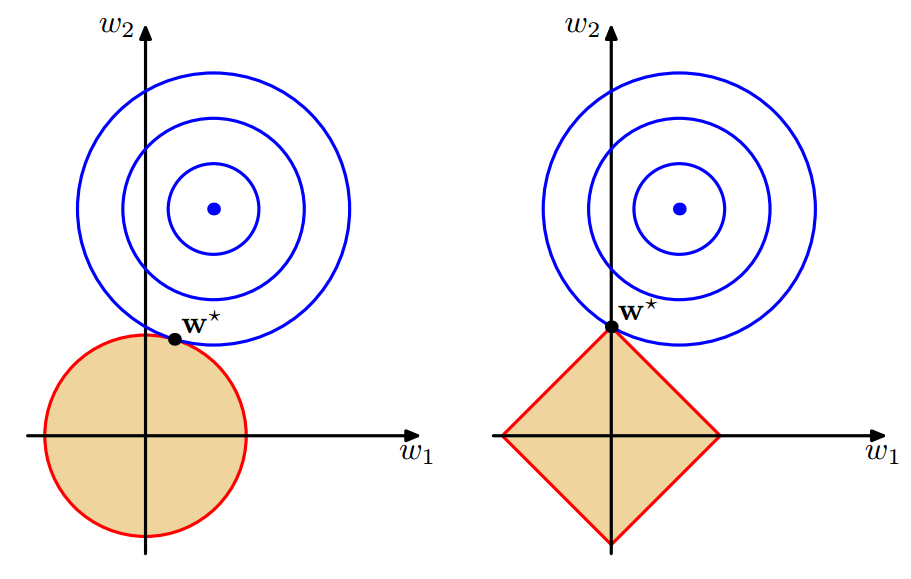
\includegraphics{D:/Documents/GitHub/Commentarii/PRML/1524666731026.png}
\caption{}
\end{figure}

Think about this figure in a Langrange-multipliers way.

\paragraph{Multiple outputs}\label{header-n81}

Of course we can decouple into multiple, independent regression
problems, however there is an approach using the same set of basis
functions so that y

\[y(x,w)=W^T\phi(x)\]

and

\[p(\mathrm{t}|x,W,\beta)=\mathcal{N}(\mathrm{t}|W^T\phi(x),\beta^{-1}I)\]

which yields

\[W_{ML}=\Phi^\dagger T\]

For the case of arbitrary covariance matrices, see MAL of multi-variate
Gaussian distribution.

\end{document}
